\section{Details of SelfAI Benchmark}
\label{sec:supp_details_benchmark}
In this section, we summarize the averaged performance across all benchmark tasks. Classical baselines, including grid search and TPE-based Bayesian optimization, achieve competitive final objective values but obtain low Scores and high $\text{AUP}_D$, reflecting redundant late-stage exploration and delayed stopping (Table~\ref{tab:hit}). Naive LLM solvers improve early discovery in some tasks but exhibit substantial variability across domains. In contrast, SelfAI-driven solvers based on mid-sized models, such as Qwen2.5-7B and GPT4-o3-mini, consistently achieve the highest Scores with substantially lower $\text{AUP}_D$ and earlier stopping times, indicating more focused and efficient discovery trajectories. Larger models (e.g., Qwen2.5-72B and Llama3.3-70B) do not necessarily yield improved efficiency, highlighting that trajectory-aware reasoning within SelfAI play a more critical role than model scale. For completeness, we discuss representative atypical trajectory behaviors in the Results section, while corresponding examples are provided. These cases illustrate exploration behaviors and breakdown patterns observed in SelfAI Benchmark, including premature stopping, limited integration of earlier observations, and sensitivity to minor perturbations, and serve to contextualize the aggregate performance trends reported above.

\subsection{Machine Learning}
{\bf Boston house pricing prediction.} We evaluate SelfAI on the Boston housing price prediction task~\cite{boston} using a random forest regression model. A total of 162 trials were conducted across a search space defined by five hyperparameters: i.e., $\text{n-estimators}=[100, 200, 300]$, $\text{max-depth} = [\text{None}, 10, 20]$, $\text{min-samples-split}=[2, 5, 10]$, $\text{min-samples-leaf=[1,2,5]}$ and $\text{max-features}=[\text{``sqrt'', ``log2''}]$). 

As shown in Fig.~\ref{fig:bar_score_aup} and Supplementary Table~\ref{tab:Boston}, GPT-4o-mini achieves the highest overall Score (0.9811), ranking first among all evaluated solvers. This performance reflects its ability to rapidly identify high-performing configurations while terminating exploration shortly thereafter, yielding superior optimization efficiency. Within the DeepSeek-R1 family, the 32B and 7B variants rank second and third, respectively, exhibiting a favorable balance between early convergence (low Best-Time) and moderate exploration diversity among open-source models. In contrast, larger models such as DeepSeek-R1-70B and Llama3.3-70B demonstrate sustained and consistent exploration but exhibit less effective stopping behavior, leading to prolonged search trajectories and delayed convergence. Notably, nearly all solvers reach an identical and high Best Result (approximately 0.841), indicating that differences in final predictive accuracy are minimal. Instead, the primary distinction lies in how efficiently and reliably solutions are discovered, underscoring the importance of trajectory-aware reasoning and adaptive stopping in practical scientific optimization.


{\noindent\bf Sentiment analysis.} We perform experiments for sentiment analysis that focus on identifying opinions, emotions, and attitudes expressed in text. All experiments are found in~\cite{sentiment_analysis} with standard experimental settings, where pre-trained Word2Vec embeddings~\cite{word2vec} are used as input features. An LSTM network is then employed to model sentence sequences, converting them into a multi-class classification problem. This setup serves to evaluate the agent's reasoning and optimization capabilities in textual domains.
As reported in Supplementary Table~\ref{tab:LSTM}, GPT-4o-mini achieves the highest Score (0.8824), consistently identifying the optimal configuration at an early stage while maintaining a balanced level of exploration. In contrast, the DeepSeek-R1 and Qwen2.5 series exhibit substantially lower Scores, frequently showing delayed convergence or failing to reach the global optimum. Notably, the largest frontier model, GPT-4o, performs markedly worse (Score 0.2745, rank 11), despite its superior scale. This result indicates that model size alone does not guarantee effective iterative hyperparameter reasoning in recurrent neural architectures, and that disciplined trajectory reasoning combined with adaptive stopping plays a more decisive role in efficient optimization within textual learning tasks.

\subsubsection{Scientific Computing}
We selected the tensor decomposition method~\cite{tw}. The method is an important tool for high-dimensional data analysis and is crucial in applications such as data compression~\cite{li2025lossless}, computational acceleration~\cite{berezutskii2025tensor}, and multi-modal data fusion~\cite{steyaert2023multimodal}. All LLMs are provided with identical mathematical knowledge about TW decomposition generated by GPT-4o. As shown in Supplementary Table~\ref{tab:TW}, Qwen2.5 (7b and 14b) and GPT4-o3-mini perform well and rank highly. In contrast, Qwen2.5-72B exhibits reduced performance, suggesting that broader general reasoning alone may be insufficient to navigate the specific trade-offs inherent in tensor decomposition. In the DeepSeek series, although the DeepSeek-R1-7b model can't find the optimal solution, its search strategy was acceptable with a moderate Score, demonstrating its ability to perform mathematical reasoning. DeepSeek-R1-70b and GPT-4o, despite excellent search diversity and early stopping, received a mediocre score, reflecting that their exploration strategy was not well aligned with the optimization goal of tensor decomposition, possibly failing to find the optimal performance between data compression and computational efficiency.

\subsection{Computer Vision}
{\noindent\bf A. SIREN} We employed SIREN (Sinusoidal Representation Networks)~\citep{sitzmann2020implicit} to evaluate our framework on image segmentation and denoising tasks. Leveraging sine activations and coordinate-based inputs, SIREN excels at representing high-frequency signals through continuous implicit representations, making it widely used in scientific computing and physics-based problems. However, its performance is highly sensitive to hyperparameters (e.g., learning rate and regularization strength, etc.), requiring careful tuning per dataset. The unsupervised nature of SIREN further increases the risk of training instability or divergence with improper settings, making it a strong test case for SelfAI's hyperparameter optimization capability. 

Fig.~\ref{fig:siren_surface} illustrates hyperparameter search trajectories for image segmentation using SIREN (see also Supplementary Figs.~\ref{fig:siren_surface1}, \ref{fig:siren_surface2}, and \ref{fig:siren_surface3}), where the surface, smoothed from the original steep, multi-peak data, reveals distinct search behaviors. Given the same three initial points, the tree-structured Bayesian optimizer (BS) follows a spiral trajectory that underutilizes promising starting regions and fails to explore broadly, often converging to local minima. In contrast, LLM-based optimizers infer trends from evaluated points, incorporate causal reasoning, and explore more broadly to locate the global optimum efficiently. They also monitor progress and halt when improvements plateau, a capability absent in traditional methods.

Quantitative results (Supplementary Tables~\ref{tab:siren_seg}-\ref{tab:siren_denoising}) reveal distinct task-dependent performance profiles. In segmentation, DeepSeek-R1-7B achieves the highest Score (0.693) and ranks first, followed by Qwen2.5-7B and GPT-4-o3-mini. Larger models such as Qwen2.5-72B and Llama-3.3-70B rank only mid-range, indicating that scale alone does not ensure effective optimization. In denoising, the landscape shifts: Qwen2.5-72B delivers the best performance (Score 0.761), while DeepSeek-R1-14B and DeepSeek-R1-32B jointly occupy second place. Notably, models that perform well in segmentation tasks do not necessarily perform well in denoising tasks, suggesting that the effectiveness of the solver largely depends on the degree of matching between its inference strategy and the task.

{\noindent\bf B. Image Classification} We also benchmark two commonly used supervised learning methods in computer vision: Masked Autoencoder (MAE)~\cite{mae} and ResNet~\cite{resnet}. These represent fundamentally different learning paradigms where hyperparameter optimization plays a crucial role in achieving the latest performance.

{\noindent\bf Mask Autoencoder (MAE)} MAE introduces two key hyperparameters: training strategies (linear detection vs. fine-tuning) and masking rate, which are explored over a range: $ [0.10, 0.90] $ with an interval of 0.1. The masking rate directly affects the difficulty of the reconstruction task and the quality of the learning representation, while the training strategy determines how to adapt to the downstream task. In our experiments (see Supplementary Table~\ref{tab:MAE} for more details), GPT-4o-mini achieved explicit performance with efficiency, demonstrating the extraordinary ability to identify the best mask configuration and training strategies. Qwen2.5-7B achieves early convergence and disciplined stopping. The DeepSeek-R1 series shows consistent scaling behavior: performance improves from 7B to 14B to 32B, but slightly drops at 70B. In traditional solvers, GS and BS lag significantly behind LLM-based solvers, highlighting the advantages of LLM-enabled discovery. Apart from Qwen2.5-14b and DeepSeek-R1-7b, most solvers can find the optimal solution, but significant differences exist among the various methods in terms of search efficiency and convergence speed.



{\noindent\bf ResNet Family} On the ImageNet ResNet hyperparameter benchmark, LLMs in the 7B-32B range demonstrate superior optimization efficacy. The top-performing solvers, such as Qwen2.5-14B (1st), DeepSeek-R1-32B (2nd), and Qwen2.5-7B with DeepSeek-R1-14B (tied 3rd), consistently identify the optimal ResNet configuration within one or two trials, halting immediately with near-perfect sample efficiency. In contrast, larger variants from the same model families drop to middle or lower rankings, consuming over half the search budget with notably higher exploration overhead. While GPT-series models, as large-scale counterparts, still achieve competitive results, the 7B-32B class exhibits a clear advantage in balancing accuracy and efficiency. For the architectural search on ImageNet, we explored key dimensions such as depth and bottleneck design. Qwen2.5-14B attains theoretical peak performance, with its 7B and 32B versions completing further exploration efficiently. These results reflect an ability to identify ideal network configurations with minimal wasted exploration.

{\noindent\bf Large-scale benchmark} We evaluate SelfAI on the standard AutoML benchmark~\cite{zimmer2021auto} using Bayesian optimization over 2000 rounds of hyperparameter search, covering critical parameters including learning rate, batch size, network depth, and dropout rate (Supplementary Fig.~\ref{fig:LCBench_analysis}). These trials exceed the maximum token limit of GPT-family models, thereby SelfAI does not employ GPT4-o3-mini or GPT4-o3. Supplementary Fig.~\ref{fig:LCBench_analysis}a-e presents that accuracy depends on interacting hyperparameters such as weight decay, hidden-layer width, and depth, and the high-performance region is sharply localized. The optimization process using the Tree Parzen Estimator (TPE) optimizer is shown with performance fluctuations that cannot be stopped (Supplementary Fig.~\ref{fig:LCBench_analysis}f), illustrating highly sparse promising regions. Supplementary Table~\ref{tab:LCBenchmark} illustrates that leading models (DeepSeek-R1-70B, Qwen2.5-14B, and Llama3.3-70B) efficiently identify near-optimal performance by evaluating only a minimal set of candidate solutions, achieving an order-of-magnitude improvement in stop-time compared to classical methods, as promising regions are identified arising from interacting hyperparameters.

% , where accuracy depends on interacting hyperparameters such as weight decay, hidden-layer width, and depth. This structure highlights why solvers must possess strong reasoning capabilities to locate these promising configurations efficiently. It motivates the need for trajectory-aware decision-making rather than purely local refinement. 

\subsection{Medical Image Analysis}
In medical image analysis, nnU-Net~\cite{nnunet} is a landmark framework known for its strong generalization and automated design. Despite its adaptive network structure, preprocessing, and training strategies for various segmentation tasks, the exploration of novel architectures persists. To address this, nnU-Net-Revisited~\cite{nnunet_revisit} establishes a comprehensive benchmark including 19 mainstream models (CNN-based~\cite{ronneberger2015u,nnunet,roy2023mednext}, Transformer-based~\cite{vaswani2017attention,tang2022self}, and Mamba-based~\cite{gu2023mamba,ma2024u}), offering a solid basis for fair evaluation. Results are shown in Figs.~\ref{fig:bar_score_aup} and Supplementary Tables~\ref{tab:MIABench}-~\ref{tab:nnUnet}. We evaluate SelfAI on this benchmark across multiple datasets, with results summarized in Fig.~\ref{fig:bar_score_aup} and Supplementary Tables~\ref{tab:MIABench}-\ref{tab:nnUnet}. On the BTCV dataset~\cite{btcv}, SelfAI instantiated with GPT4-o3-mini achieves the highest Score (0.6875) and ranks first, indicating rapid identification of high-quality configurations combined with efficient stopping behavior. Notably, Qwen2.5-7B secures second place, outperforming all larger variants within the same model family, suggesting that effective optimization in this setting does not scale monotonically with model size. A similar pattern emerges in nnU-Net hyperparameter tuning on the BraTS dataset~\cite{brats}. Qwen2.5-14B attains the top ranking (Score 0.4333), followed closely by GPT4-o3-mini, while Qwen2.5-32B and DeepSeek-R1-70B tie for third. Across both datasets, smaller (7B) and very large (72B) models outperform medium-sized counterparts (14B-32B), reinforcing the observation that increased model capacity alone does not guarantee superior optimization performance. These results highlight the importance of trajectory-aware decision-making under noisy and high-variance evaluation regimes, which are characteristic of medical image analysis. By committing early to promising configurations while avoiding prolonged exploration with diminishing returns, SelfAI enables efficient discovery in settings where excessive experimentation is both computationally costly and practically constrained.

\subsection{Imbalanced Node Classification}
Graph neural networks (GNNs) are a central modeling paradigm for relational data and have become indispensable across a range of scientific domains. In biomedicine, GNNs underpin modern protein structure prediction systems, such as AlphaFold3, by enabling explicit modeling of spatial interactions among amino acid residues, thereby advancing structural biology at unprecedented resolution~\cite{alphafold3}. In drug discovery, GNNs are widely applied to molecular property prediction, compound-target interaction modeling, and de novo molecule generation~\cite{bongini2021molecular}. Despite their success, optimizing GNNs on imbalanced datasets remains particularly challenging, due to sparse and asymmetric reward signals, complex relational dependencies, and high-dimensional hyperparameter spaces. These characteristics make such tasks especially sensitive to exploration strategy and stopping decisions. To investigate whether trajectory-aware reasoning can address these challenges, we evaluate GraphSAGE on the imbalanced Cora benchmark~\cite{zhao2021graphsmote} under the setup~\cite{yan2023unreal}.

As shown in Fig.~\ref{fig:bar_score_aup}, SelfAI instantiated with the GPT4-o3 series consistently achieves near-optimal performance, characterized by rapid identification of optimal configurations, efficient stopping decisions, and sustained exploration diversity. This behavior indicates that SelfAI effectively balances exploitation and exploration in structurally complex optimization landscapes. In contrast, Qwen2.5 models (with the exception of the 72B variant) exhibit stable but middling performance across scales, while larger models tend to converge later and incur substantial redundant exploration. This pattern suggests potential limitations in capturing the structural optimization requirements of relational domains such as molecular graphs and protein interaction networks (see Supplementary Table~\ref{tab:GraphSAGE}). Across different language model backbones, SelfAI consistently demonstrates fast discovery of high-quality configurations while avoiding premature convergence. These results provide evidence that trajectory-level reasoning and adaptive stopping generalize beyond continuous parameter optimization, extending effectively to structured, relational learning problems that are common in real-world scientific applications.

\subsection{Drug Discovery}
Drug discovery increasingly benefits from advances in machine learning and data-driven modeling, which serve as versatile frameworks for tasks such as bioactivity prediction, virtual screening, and compound prioritization. These approaches have demonstrated the potential to accelerate early-stage discovery, reduce experimental burden, and shorten development timelines~\cite{brahmavar2024generating,grisoni2021combining}. Following the evaluation practices and modeling standards summarized by Korotcov et al.~\cite{korotcov2017comparison}, this study employs the Chagas EP20 dataset~\cite{Chagas}, which measures the activity of compounds against Trypanosoma cruzi, a neglected but medically significant target in tropical disease research. The core challenge lies in learning an effective mapping from molecular representations, such as SMILES sequences~\cite{weininger1988smiles}, to experimentally measured bioactivity~\cite{fliri2005biological}. We adopt SelfAI to adaptively refine model performance, monitor discovery trajectories, and determine principled stopping criteria for iterative optimization. Experimental results (see Supplementary Table~\ref{tab:chagas}) reveal distinct performance patterns among solvers in hyperparameter optimization. SelfAI and select LLM-based solvers achieve superior Scores by rapidly identifying promising hyperparameter regions and terminating exploration once gains plateau. Notably, these results demonstrate efficient optimization under realistic biochemical uncertainty, highlighting trajectory-aware optimization as a practical computational enabler for scalable and resource-efficient bioactivity modeling in drug discovery pipelines.

% We additionally include in Supplementary Fig.~\ref{fig:selfai_metrics} a decomposition of solver behavior across Avg Improvement, Stop Time, Best-Time, Score, and $\text{AUP}_D$
% , providing the full technical breakdown underlying the results shown in the main paper.



% \begin{figure}
%     \centering
%     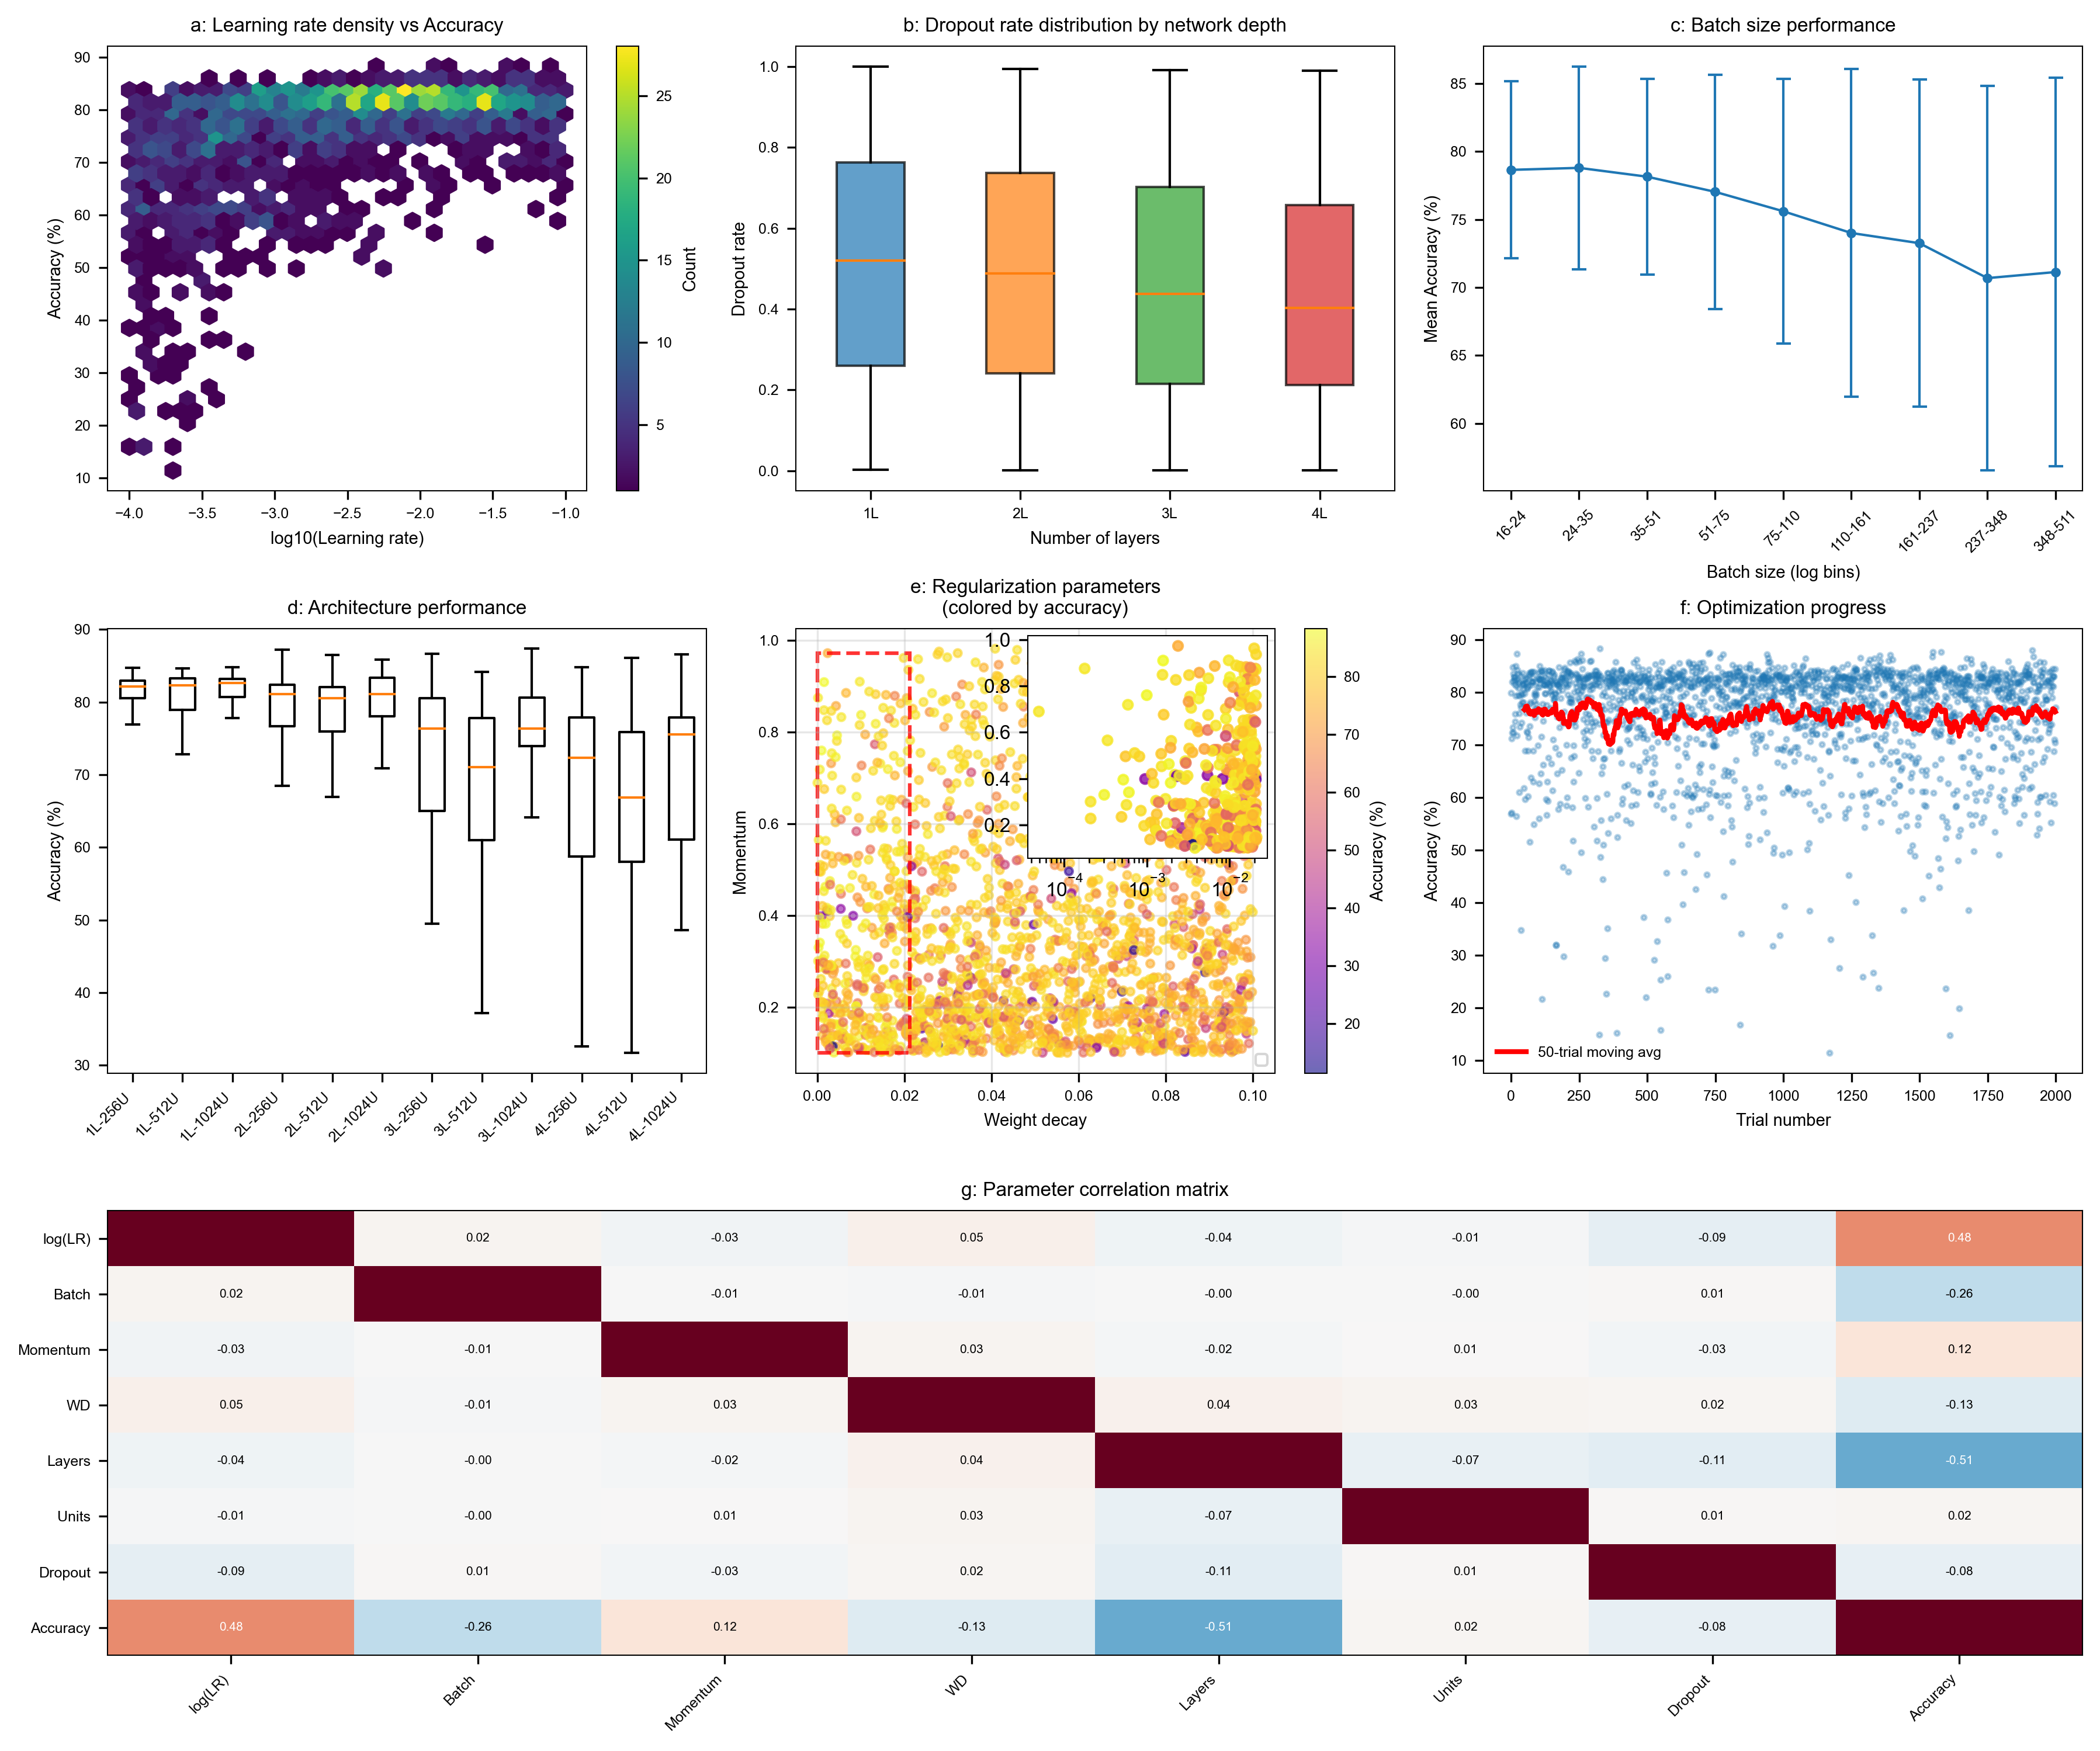
\includegraphics[width=1.0\linewidth]{figures/analysis/LCBench_comprehensive_analysis.png}
%     \caption{The relationship between different parameter settings and accuracy. \textbf{a}, A hexbin plot showing the joint density of learning rate (log-scaled) and accuracy. \textbf{b}, Box plots illustrating the distribution of dropout rates used for models of different depths. \textbf{c}, Mean accuracy and standard error across logarithmically binned batch sizes. \textbf{d}, Performance comparison of different architectural configurations (layers and units). \textbf{e}, A scatter plot of weight decay against momentum, colored by accuracy. \textbf{f}, The optimization trajectory, showing accuracy improvement over successive trials, with a moving average trend line. \textbf{g} A correlation matrix quantifying linear relationships between all parameters and the accuracy.}
%     \label{fig:LCBench_analysis}
% \end{figure}


% \subsection{Performance Discussion}
% \label{sec:supp_discussion}
% In Supplementary Fig.~\ref{fig:breakthrough_points}, we present breakthrough points to analyze the optimization trajectory. LLM-powered solvers commonly discover more breakthrough points at an early stage. Lower mean values of breakthrough positions represent a highly effective exploration strategy. In addition, the figure demonstrates the consistency between the Score and the breakthrough points.


% Then, in Supplementary Figs.~\ref{fig:bar_score} and ~\ref{fig:bar_aup}, we further report Score and $\text{AUP}_D$ metrics for each task. A higher Score can be obtained by LLM-powered solvers. 




\begin{figure}
    \centering
    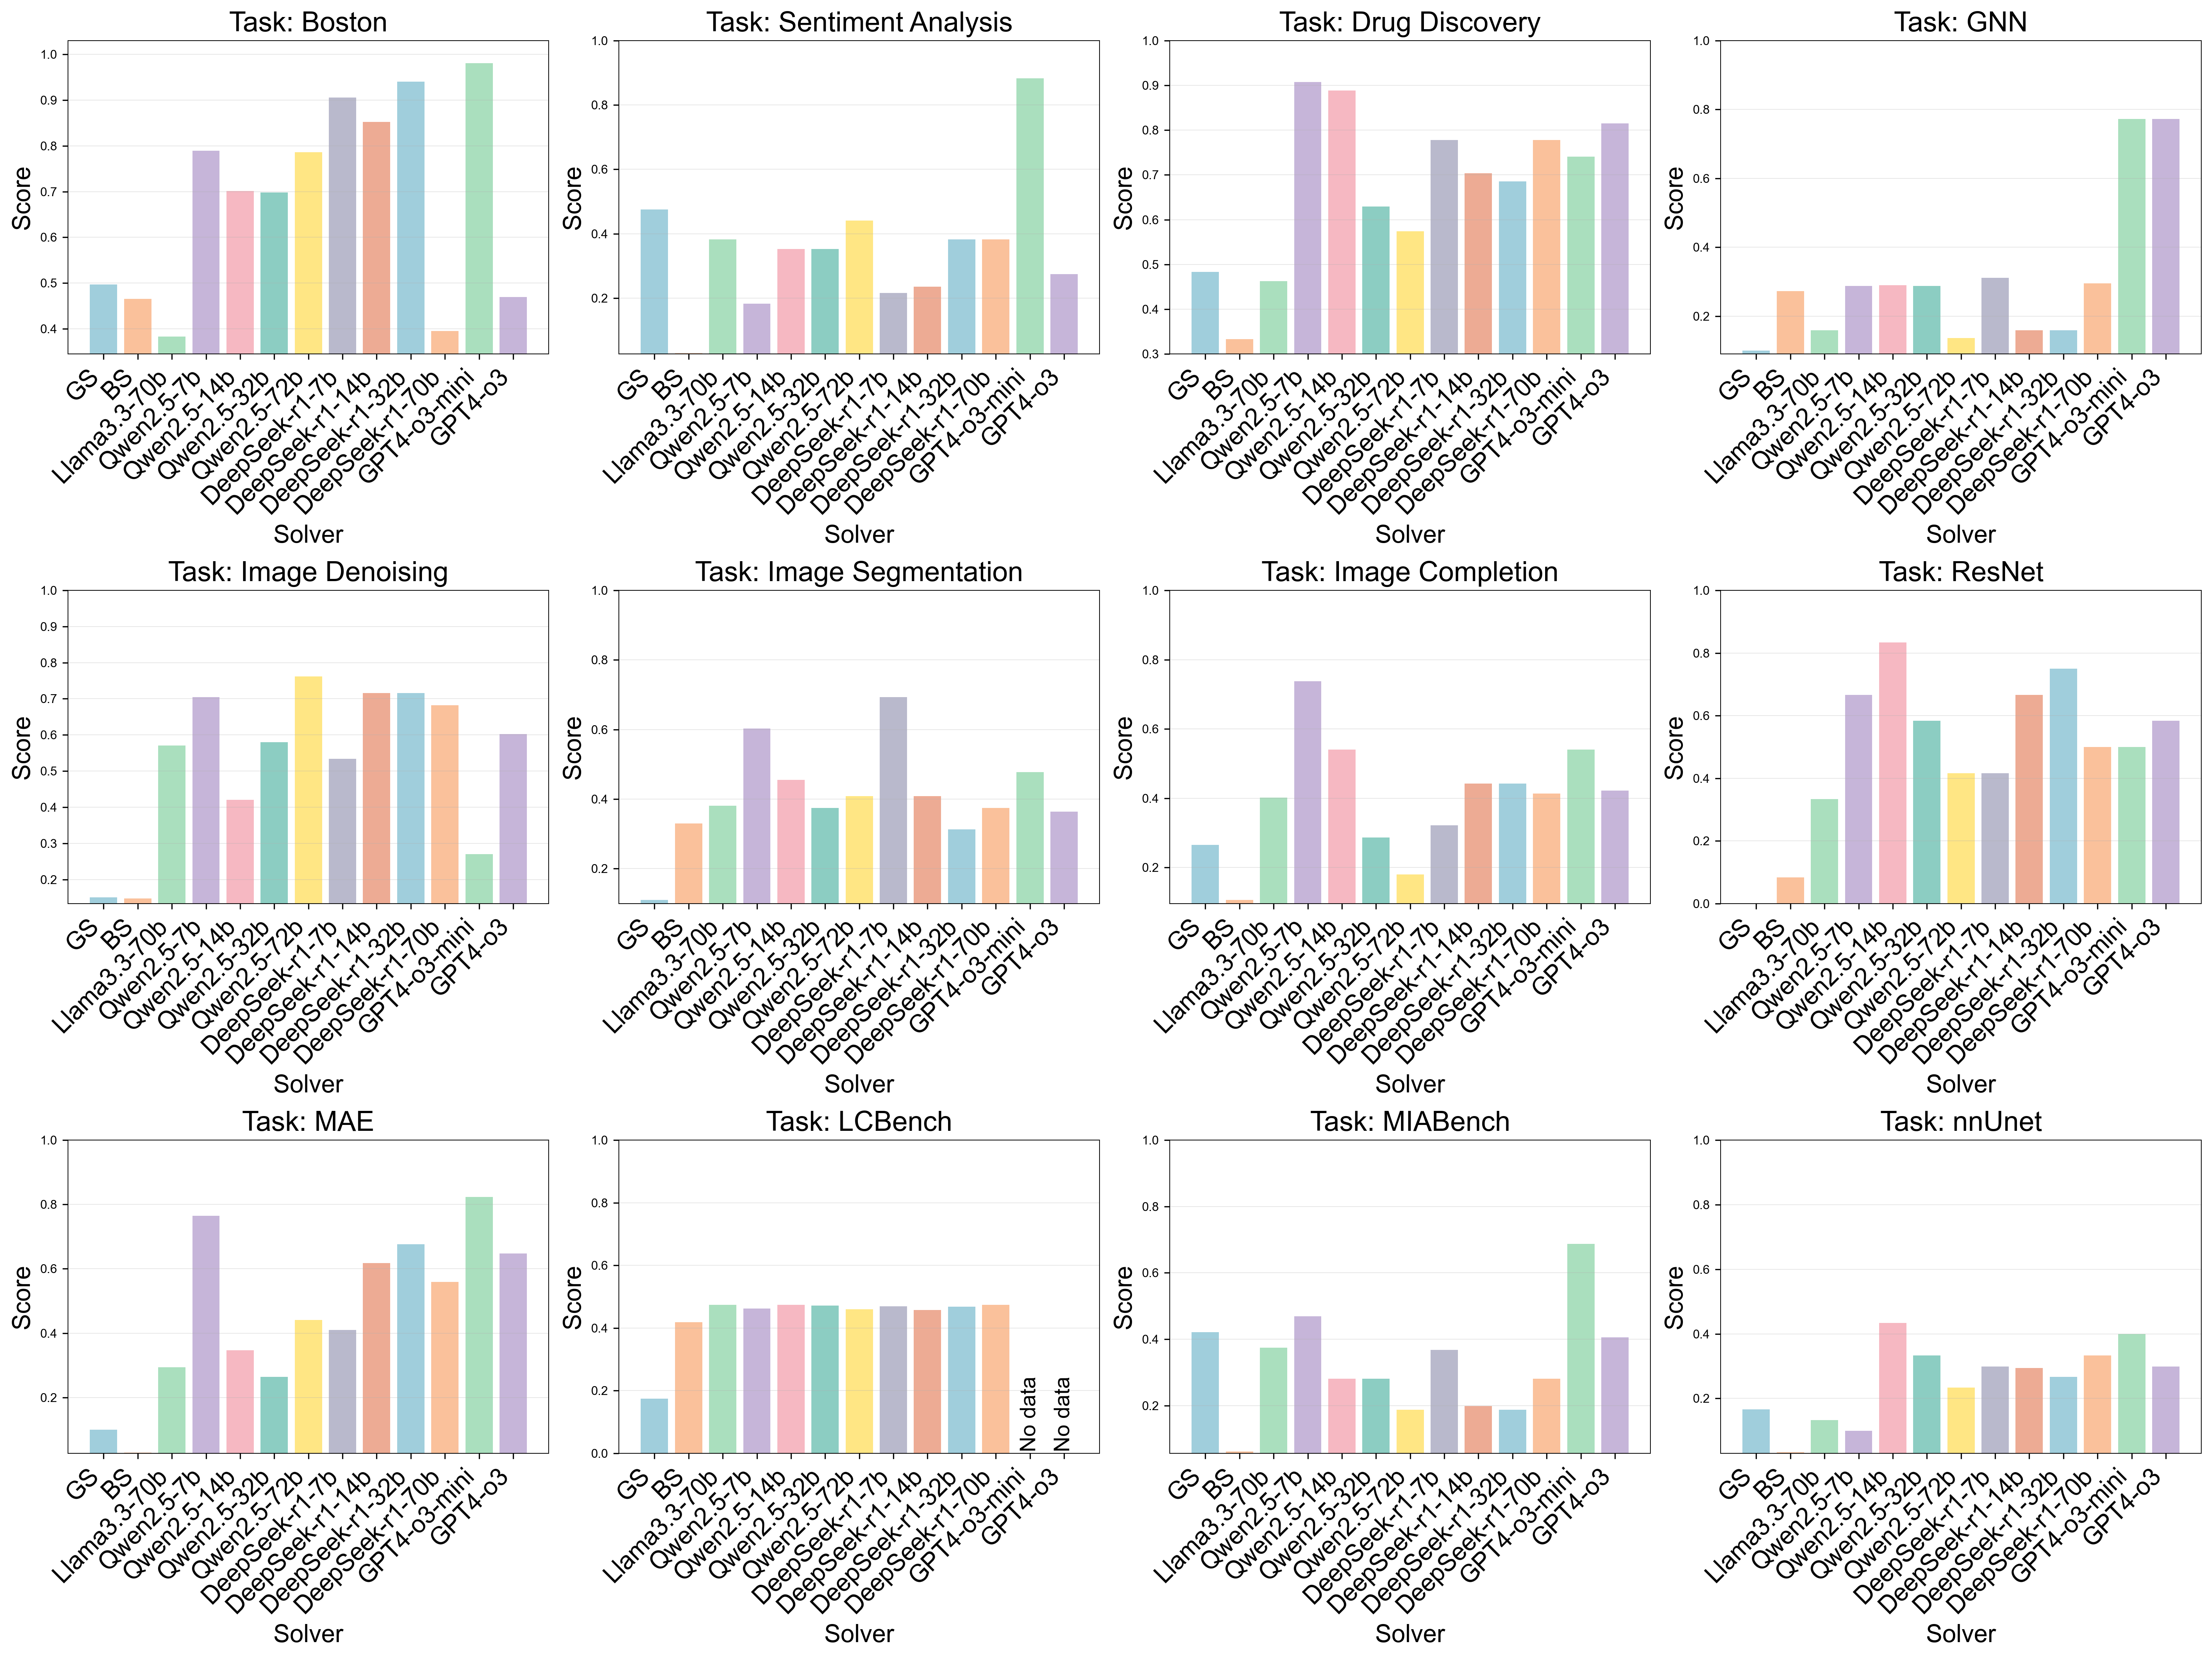
\includegraphics[width=0.9\linewidth]{figures/analysis/separate_bar_charts_score.png} \\
    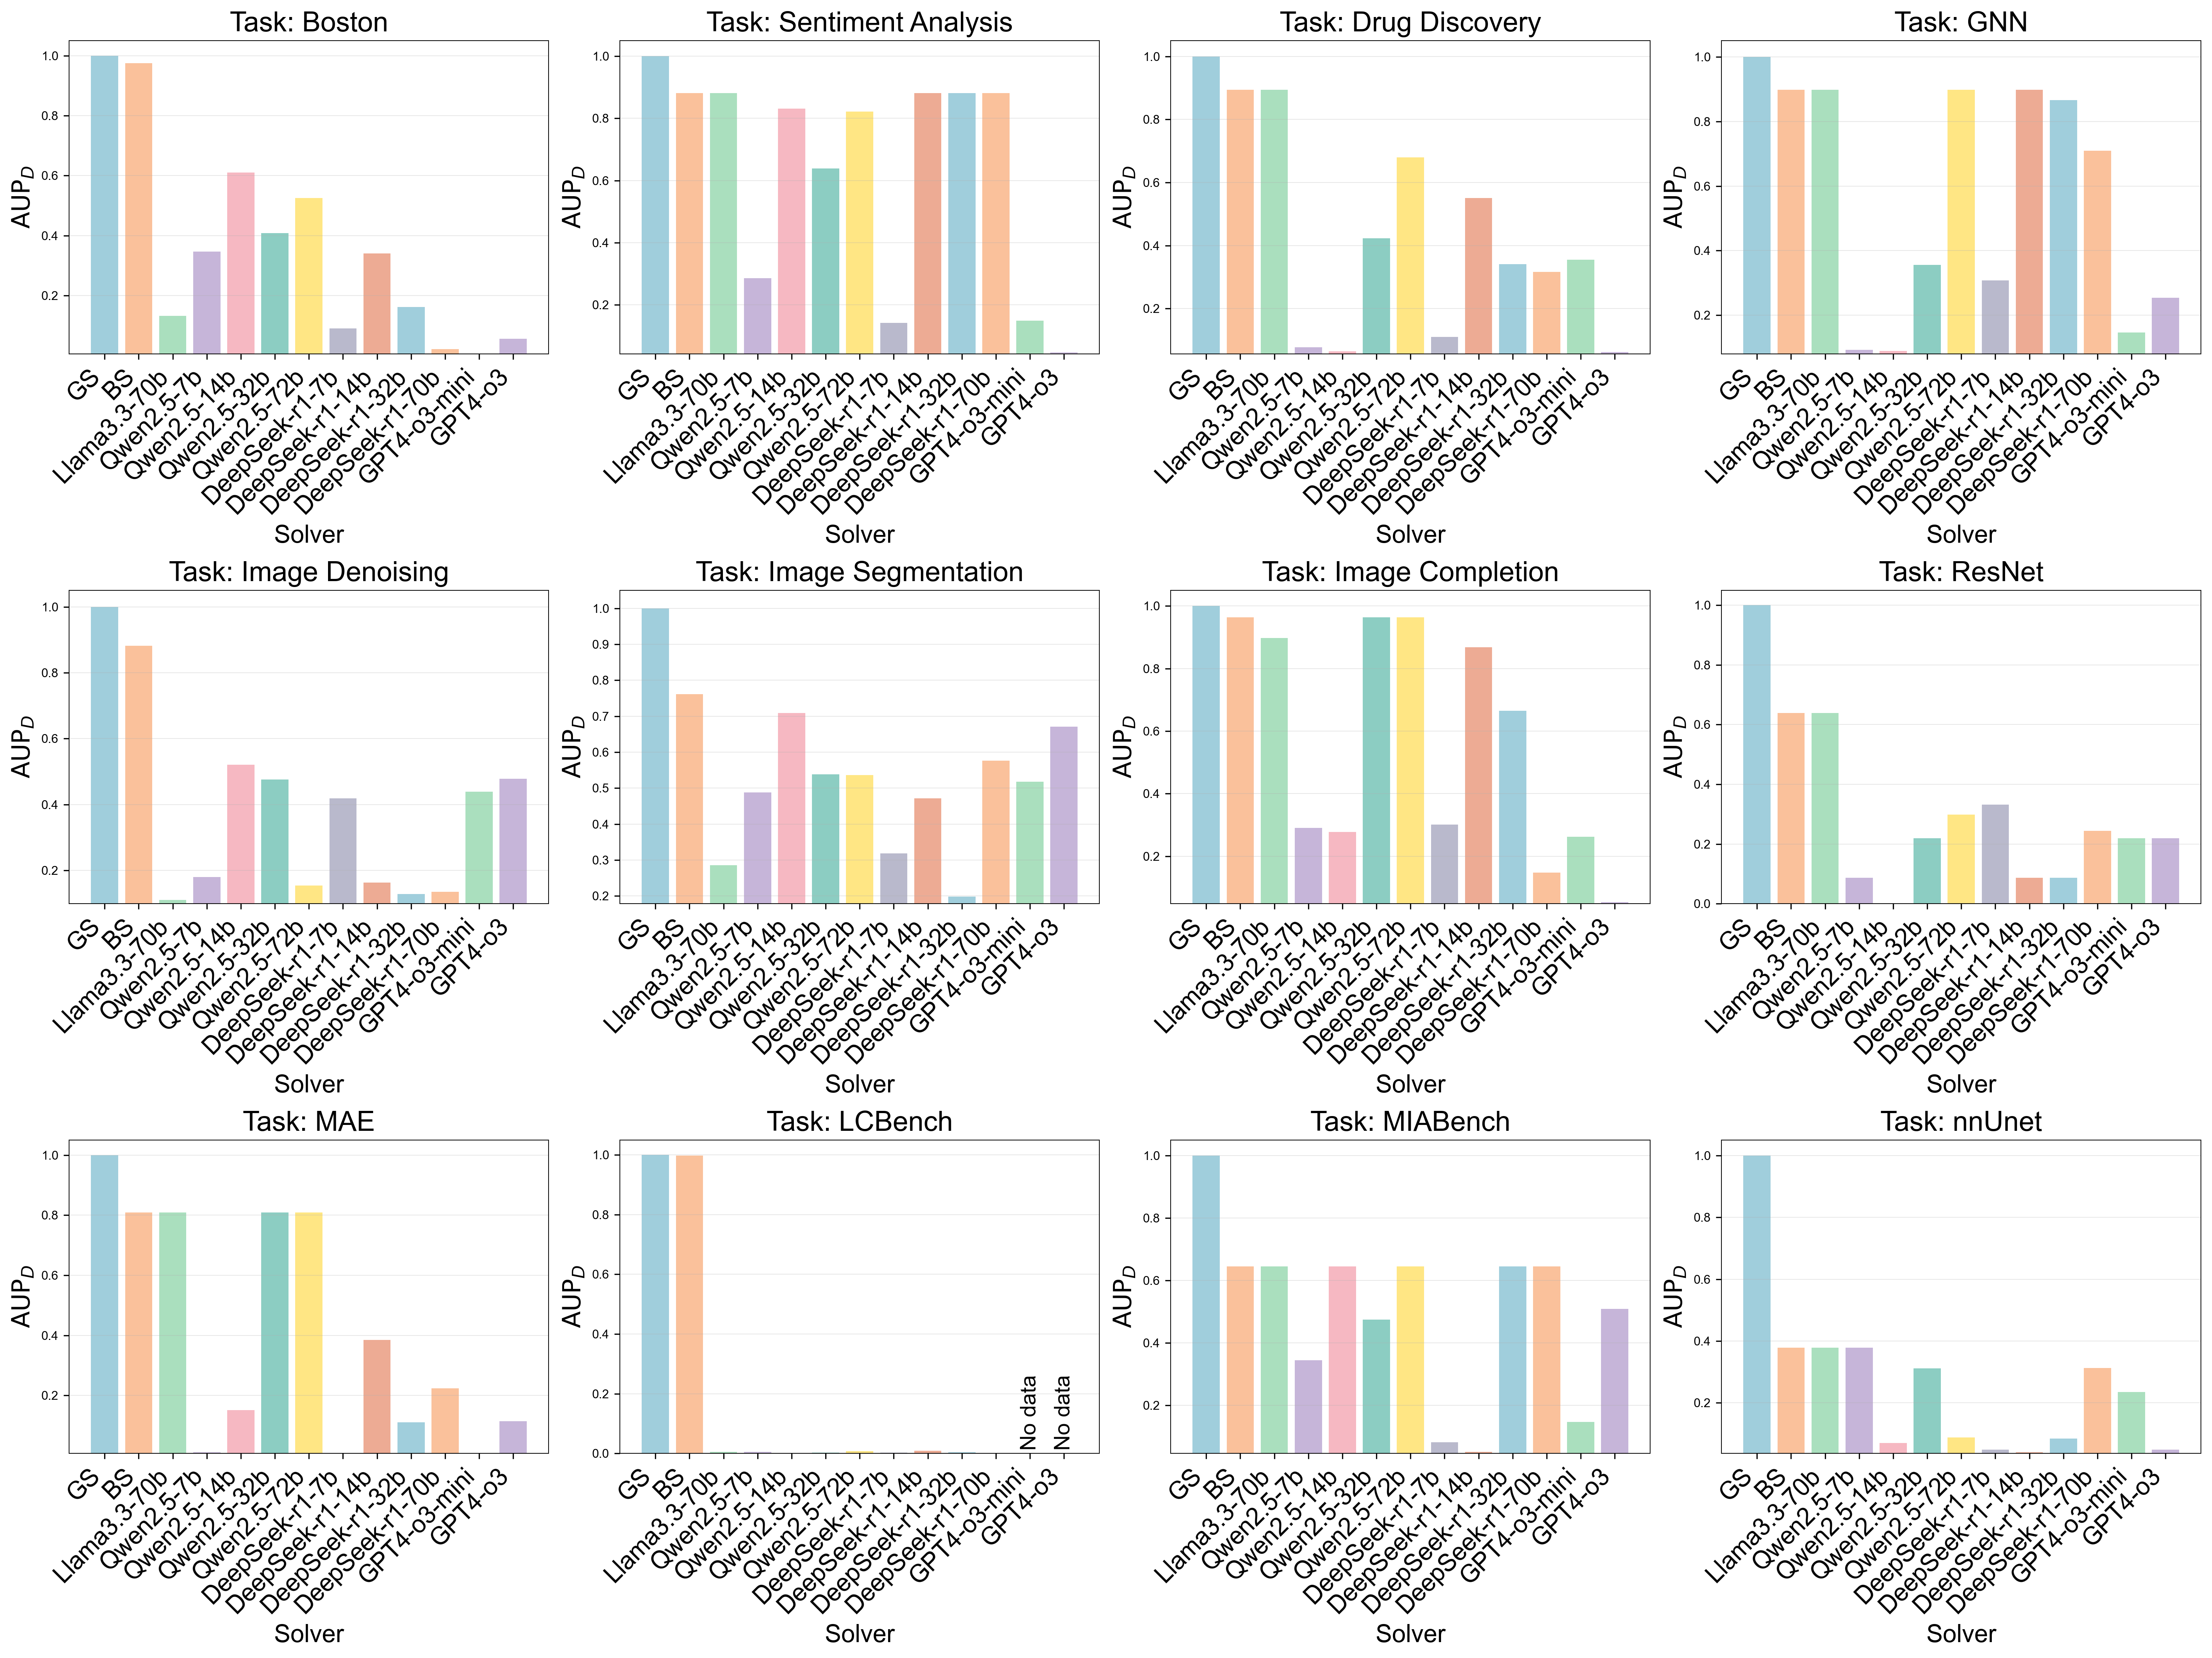
\includegraphics[width=0.9\linewidth]{figures/analysis/separate_bar_charts_aup.png}
    \caption{The top three rows present the Score of all solvers across different tasks, which assess the best stopping performance of SelfAI and baselines using different LLMs. The bottom three rows present the Diverse Metrics ($\text{AUP}_D$) of all solvers across different tasks, evaluating the diversity of solution trajectories. }
    \label{fig:bar_score_aup}
\end{figure}






\begin{figure}
    \centering
    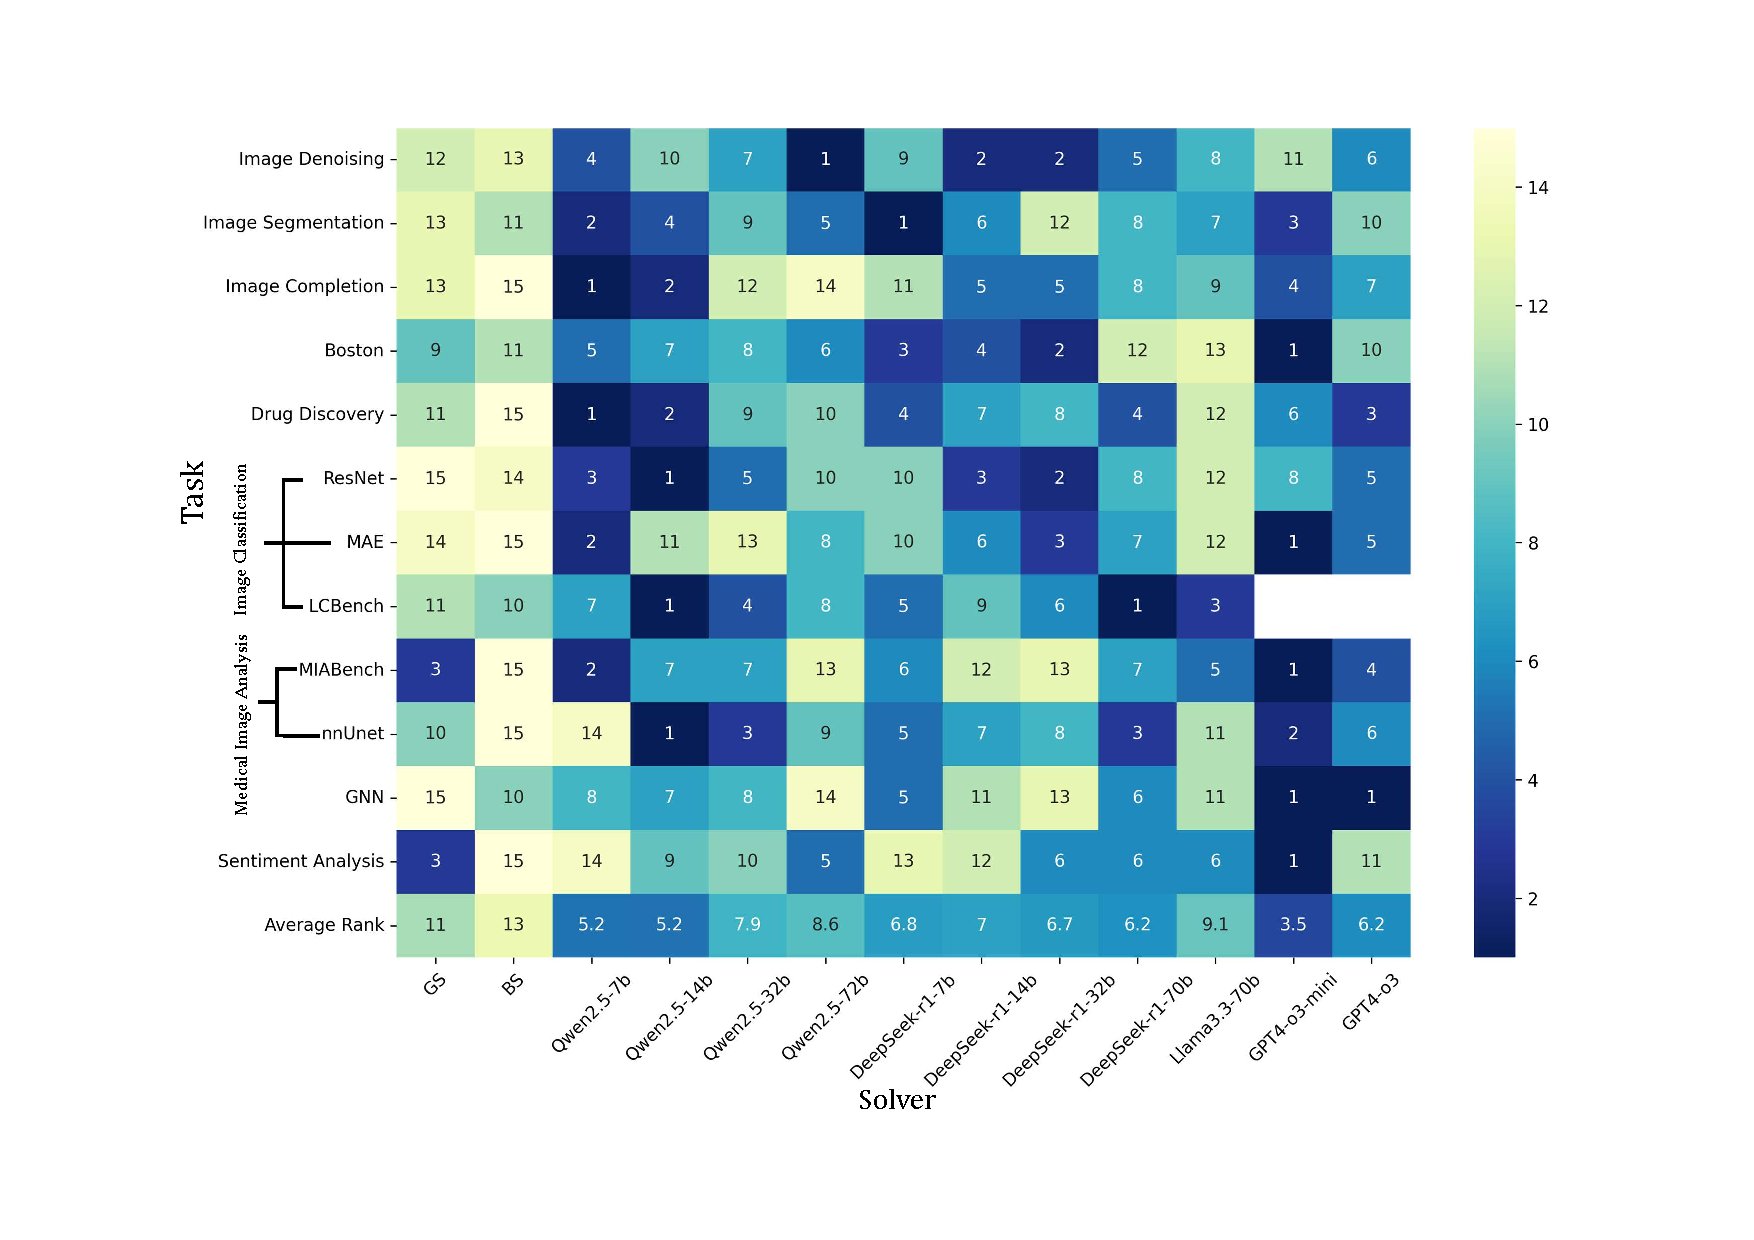
\includegraphics[width=1.0\linewidth]{figures/analysis/rank_heatmap.pdf}
    \caption{Performance ranking of different methods across multiple tasks. The heatmap displays the rank of each method (rows) for every task (columns), where lower numbers (darker colors) indicate better performance (e.g., 1st place). The final average rank is summarized on the right.}
    \label{fig:rank_heatmap}
\end{figure}




\begin{figure*}[t]
    \centering
    \begin{tabular}{cccc}

        \multicolumn{4}{c}{\textbf{BS}} \\
        
\includegraphics[width=0.22\textwidth]{figures/siren/siren_cameraman_TV/bayes.png}
        & 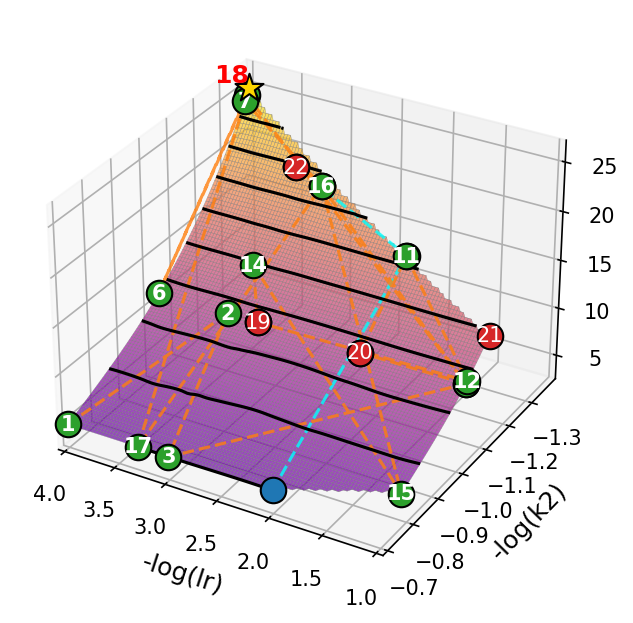
\includegraphics[width=0.22\textwidth]{figures/siren/siren_cameraman_FH/bayes.png}
        & 
\includegraphics[width=0.22\textwidth]{figures/siren/siren_cat_me3_TV/bayes.png}
        & 
\includegraphics[width=0.22\textwidth]{figures/siren/siren_cat_me3_FH/bayes.png}\\

        \multicolumn{4}{c}{\textbf{GPT4-o3-mini}} \\
        
\includegraphics[width=0.22\textwidth]{figures/siren/siren_cameraman_TV/GPT4-o3-mini.png}
        & 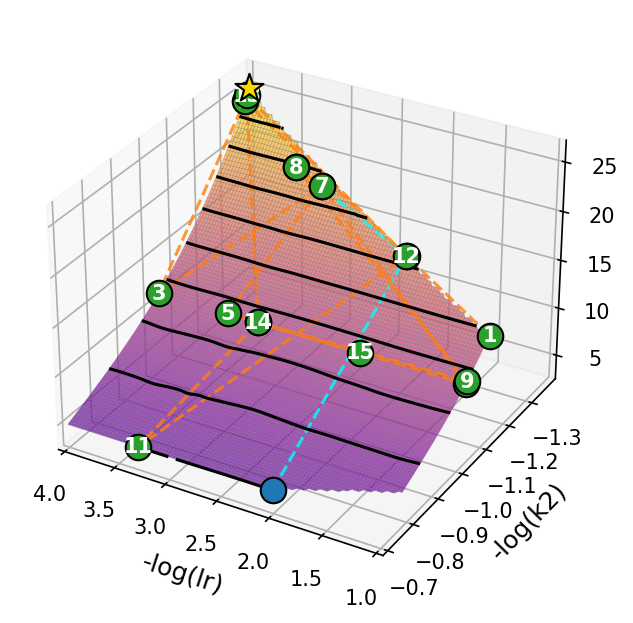
\includegraphics[width=0.22\textwidth]{figures/siren/siren_cameraman_FH/GPT4-o3-mini.png}
        & 
\includegraphics[width=0.22\textwidth]{figures/siren/siren_cat_me3_TV/GPT4-o3-mini.png}
        & 
\includegraphics[width=0.22\textwidth]{figures/siren/siren_cat_me3_FH/GPT4-o3-mini.png} \\


        \multicolumn{4}{c}{\textbf{GPT4-o3}} \\
        
\includegraphics[width=0.22\textwidth]{figures/siren/siren_cameraman_TV/GPT4-o3.png}
        & 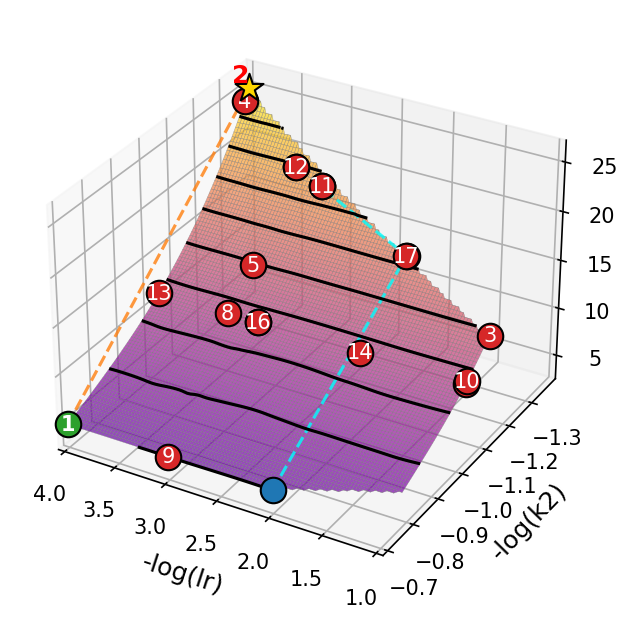
\includegraphics[width=0.22\textwidth]{figures/siren/siren_cameraman_FH/GPT4-o3.png}
        & 
\includegraphics[width=0.22\textwidth]{figures/siren/siren_cat_me3_TV/GPT4-o3.png}
        & 
\includegraphics[width=0.22\textwidth]{figures/siren/siren_cat_me3_FH/GPT4-o3.png} \\

        \multicolumn{4}{c}{\textbf{Llama3.3-70B}} \\
        
\includegraphics[width=0.22\textwidth]{figures/siren/siren_cameraman_TV/Llama3.3_70b.png}
        & 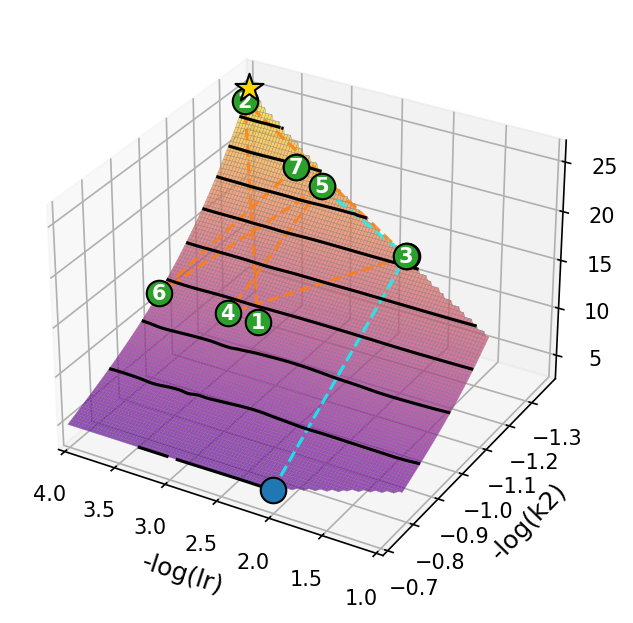
\includegraphics[width=0.22\textwidth]{figures/siren/siren_cameraman_FH/Llama3.3_70b.png}
        & 
\includegraphics[width=0.22\textwidth]{figures/siren/siren_cat_me3_TV/Llama3.3_70b.png}
        & 
\includegraphics[width=0.22\textwidth]{figures/siren/siren_cat_me3_FH/Llama3.3_70b.png} \\
    \end{tabular}
    \caption{Illustration of the optimized trajectory using the SIREN method for additional cases in image denoising (first two columns) and segmentation (last two columns). Blue points are initial points. Green points represent suggested points before reaching the optimum. Red points indicate redundant suggestions generated after the optimal point has been reached. The $\star$ marks the optimal point. The numbered labels indicate the sequence of recommendations provided by LLMs.}
    \label{fig:siren_surface1}
\end{figure*}

\begin{figure*}[t]
    \centering
    \begin{tabular}{cccc}
        \multicolumn{4}{c}{\textbf{Qwen2.5-7B}} \\
        
\includegraphics[width=0.22\textwidth]{figures/siren/siren_cameraman_TV/Qwen2.5_7b.png}
        & 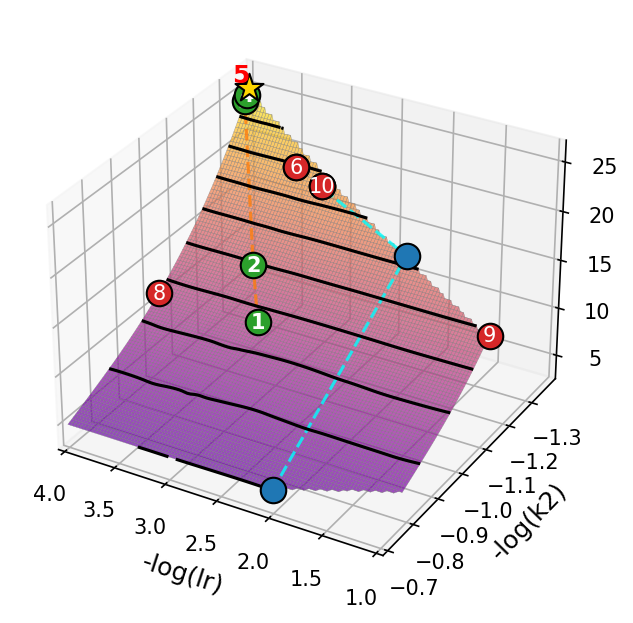
\includegraphics[width=0.22\textwidth]{figures/siren/siren_cameraman_FH/Qwen2.5_7b.png}
        & 
\includegraphics[width=0.22\textwidth]{figures/siren/siren_cat_me3_TV/Qwen2.5_7b.png}
        & 
\includegraphics[width=0.22\textwidth]{figures/siren/siren_cat_me3_FH/Qwen2.5_7b.png} \\

        \multicolumn{4}{c}{\textbf{Qwen2.5-14B}} \\
        
\includegraphics[width=0.22\textwidth]{figures/siren/siren_cameraman_TV/Qwen2.5_14b.png}
        & 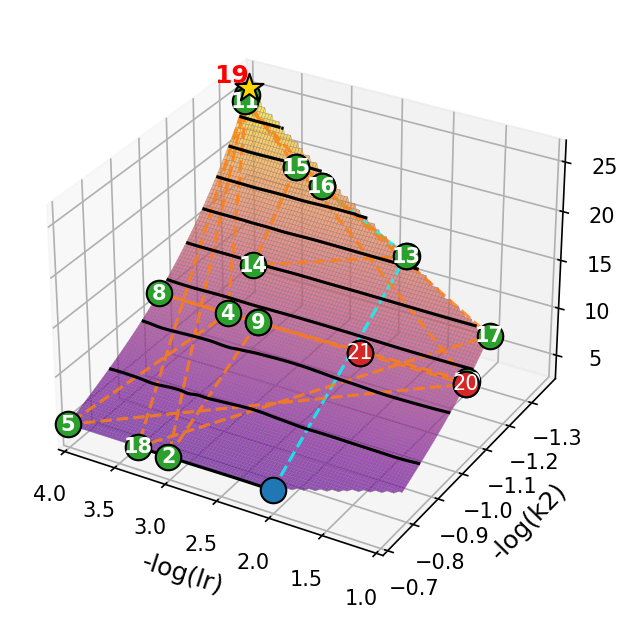
\includegraphics[width=0.22\textwidth]{figures/siren/siren_cameraman_FH/Qwen2.5_14b.png}
        & 
\includegraphics[width=0.22\textwidth]{figures/siren/siren_cat_me3_TV/Qwen2.5_14b.png}
        & 
\includegraphics[width=0.22\textwidth]{figures/siren/siren_cat_me3_FH/Qwen2.5_14b.png} \\

        
        \multicolumn{4}{c}{\textbf{Qwen2.5-72B}} \\
        
\includegraphics[width=0.22\textwidth]{figures/siren/siren_cameraman_TV/Qwen2.5_32b.png}
        & 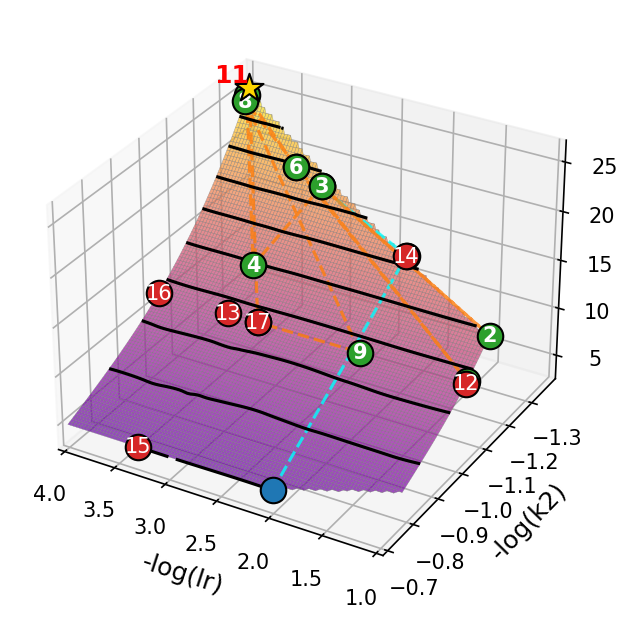
\includegraphics[width=0.22\textwidth]{figures/siren/siren_cameraman_FH/Qwen2.5_32b.png}
        & 
\includegraphics[width=0.22\textwidth]{figures/siren/siren_cat_me3_TV/Qwen2.5_32b.png}
        & 
\includegraphics[width=0.22\textwidth]{figures/siren/siren_cat_me3_FH/Qwen2.5_32b.png} \\
    
        \multicolumn{4}{c}{\textbf{Qwen2.5-72B}} \\
        
\includegraphics[width=0.22\textwidth]{figures/siren/siren_cameraman_TV/Qwen2.5_72b.png}
        & 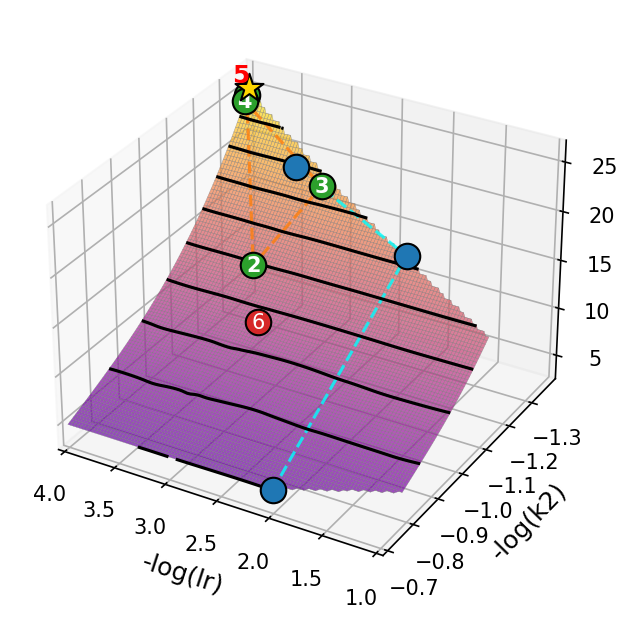
\includegraphics[width=0.22\textwidth]{figures/siren/siren_cameraman_FH/Qwen2.5_72b.png}
        & 
\includegraphics[width=0.22\textwidth]{figures/siren/siren_cat_me3_TV/Qwen2.5_72b.png}
        & 
\includegraphics[width=0.22\textwidth]{figures/siren/siren_cat_me3_FH/Qwen2.5_72b.png} \\
    \end{tabular}
    \caption{More optimized trajectories of Fig.~\ref{fig:siren_surface1}. }
    \label{fig:siren_surface2}
\end{figure*}


\begin{figure*}[t]
    \centering
    \begin{tabular}{cccc}
        \multicolumn{4}{c}{\textbf{DeepSeek-R1-7B}} \\
        
\includegraphics[width=0.22\textwidth]{figures/siren/siren_cameraman_TV/DeepSeek-r1_7b.png}
        & 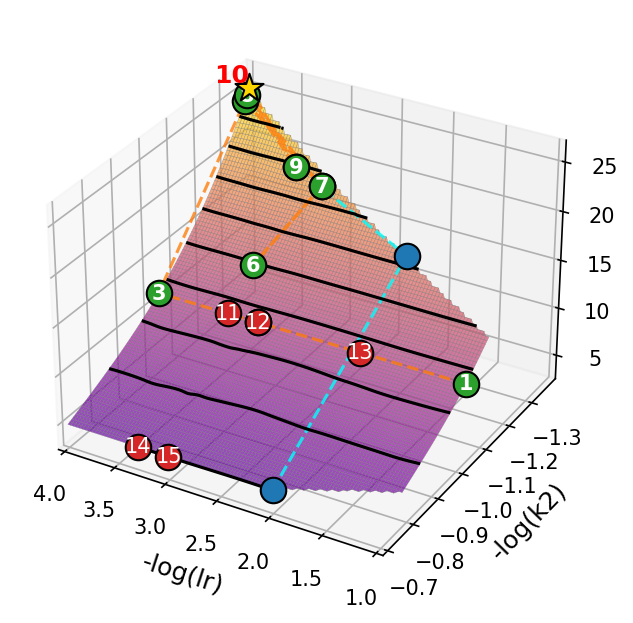
\includegraphics[width=0.22\textwidth]{figures/siren/siren_cameraman_FH/DeepSeek-r1_7b.png}
        & 
\includegraphics[width=0.22\textwidth]{figures/siren/siren_cat_me3_TV/DeepSeek-r1_7b.png}
        & 
\includegraphics[width=0.22\textwidth]{figures/siren/siren_cat_me3_FH/DeepSeek-r1_7b.png} \\

        \multicolumn{4}{c}{\textbf{DeepSeek-R1-14B}} \\
        
\includegraphics[width=0.22\textwidth]{figures/siren/siren_cameraman_TV/DeepSeek-r1_14b.png}
        & 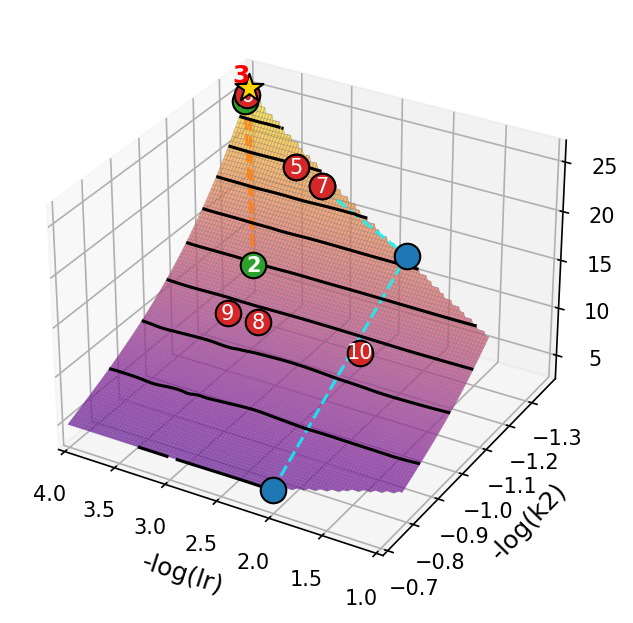
\includegraphics[width=0.22\textwidth]{figures/siren/siren_cameraman_FH/DeepSeek-r1_14b.png}
        & 
\includegraphics[width=0.22\textwidth]{figures/siren/siren_cat_me3_TV/DeepSeek-r1_14b.png}
        & 
\includegraphics[width=0.22\textwidth]{figures/siren/siren_cat_me3_FH/DeepSeek-r1_14b.png} \\

        
        \multicolumn{4}{c}{\textbf{DeepSeek-R1-32B}} \\
        
\includegraphics[width=0.22\textwidth]{figures/siren/siren_cameraman_TV/DeepSeek-r1_32b.png}
        & 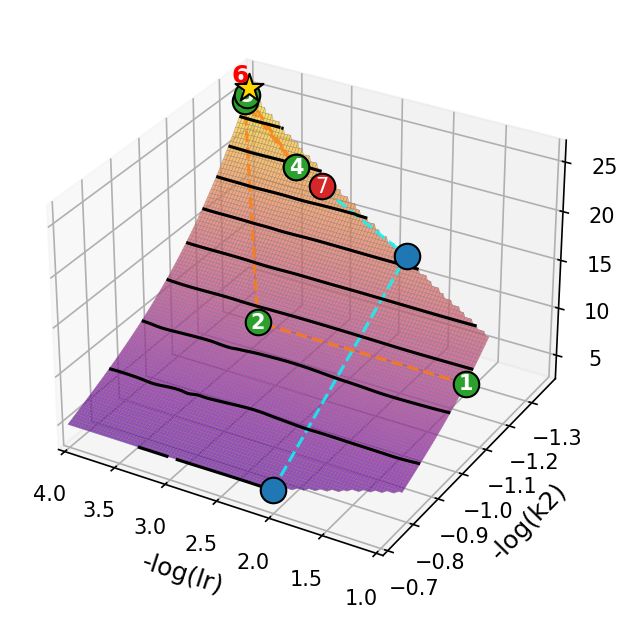
\includegraphics[width=0.22\textwidth]{figures/siren/siren_cameraman_FH/DeepSeek-r1_32b.png}
        & 
\includegraphics[width=0.22\textwidth]{figures/siren/siren_cat_me3_TV/DeepSeek-r1_32b.png}
        & 
\includegraphics[width=0.22\textwidth]{figures/siren/siren_cat_me3_FH/DeepSeek-r1_32b.png} \\
    
        \multicolumn{4}{c}{\textbf{DeepSeek-R1-70B}} \\
        
\includegraphics[width=0.22\textwidth]{figures/siren/siren_cameraman_TV/DeepSeek-r1_70b.png}
        & 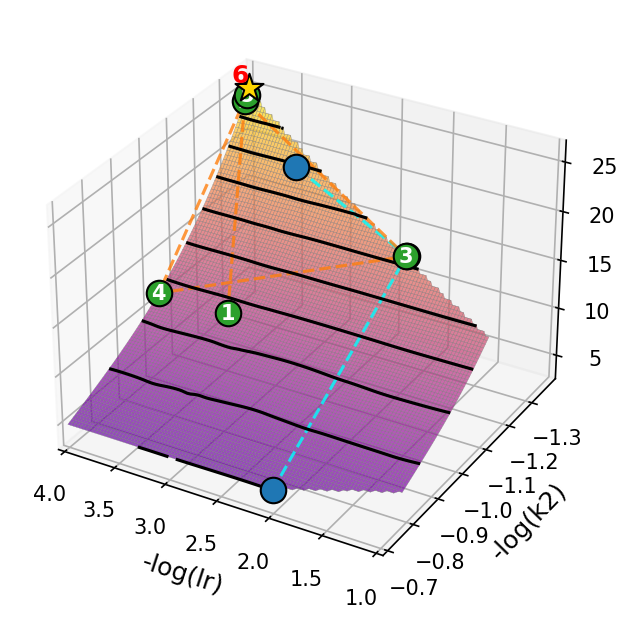
\includegraphics[width=0.22\textwidth]{figures/siren/siren_cameraman_FH/DeepSeek-r1_70b.png}
        & 
\includegraphics[width=0.22\textwidth]{figures/siren/siren_cat_me3_TV/DeepSeek-r1_70b.png}
        & 
\includegraphics[width=0.22\textwidth]{figures/siren/siren_cat_me3_FH/DeepSeek-r1_70b.png} \\
    \end{tabular}
    \caption{More optimized trajectories of Fig.~\ref{fig:siren_surface1}. These LLMs have different suggestions for non-convex hyperparameter optimization. }
    \label{fig:siren_surface3}
\end{figure*}

\subsection{Limitations}
\label{sec:supp_limitations}
\noindent\textbf{1) Context limitations.}
LCBench contains approximately 2000 trials, constituting a large and highly sparse search space. Performance depends on interacting hyperparameters such as weight decay, hidden-layer width, and depth, and high-performing regions are sharply localized. In practice, such large and sparse search spaces are common in scientific discovery tasks and can exceed the maximum context length supported by current GPT-family models.

2) {\noindent\bf Computational fragility.} Supplementary Table~\ref{tab:hit} compares the best result hit rates across solvers. The performance of LLM-based solvers is highly sensitive to the reasoning strategy, and early stopping often leads to a decline in hit rate. In the supplementary tables, we report the best result \( t_{\text{best}} \) for each solver. \( t_{\text{best}} = 1 \) indicates that the optimal result was not found. Moreover, when \( t_{\text{best}} = 1 \), the score metric improves significantly, highlighting the solver's weakness in optimal stopping. As illustrated in Fig.~\ref{fig:failure_case}, computational fragility also hinders reliable performance improvement through parameter tuning, as seen in the non-monotonic performance of the DeepSeek-R1 model series.

3) {\noindent\bf Insufficient trajectory integration.} Supplementary Fig.~\ref{fig:failure_case} provides representative trajectory visualizations that highlight differences in evidence integration and stopping behavior. The Qwen2.5 models typically identify high-performing configurations early, with Qwen2.5-7B reaching near-optimal regions within the first 10-15 trials, followed by stable refinement with limited oscillation. In contrast, DeepSeek-R1 trajectories are more frequently non-monotonic. DeepSeek-R1-7B often oscillates between high- and low-performing regions, indicating instability in how accumulated evidence is leveraged, while DeepSeek-R1-70B can terminate prematurely after early improvements, leaving promising regions under-refined. Classical baselines (GS and BS) may also reach high-performing regions, but their improvements tend to be slower and less punctuated by rapid breakthroughs. Overall, these examples complement the aggregate metrics in the main text by illustrating how limitations can manifest as reduced trajectory stability, delayed breakthroughs, or suboptimal stopping decisions.

\begin{figure}
    \centering
    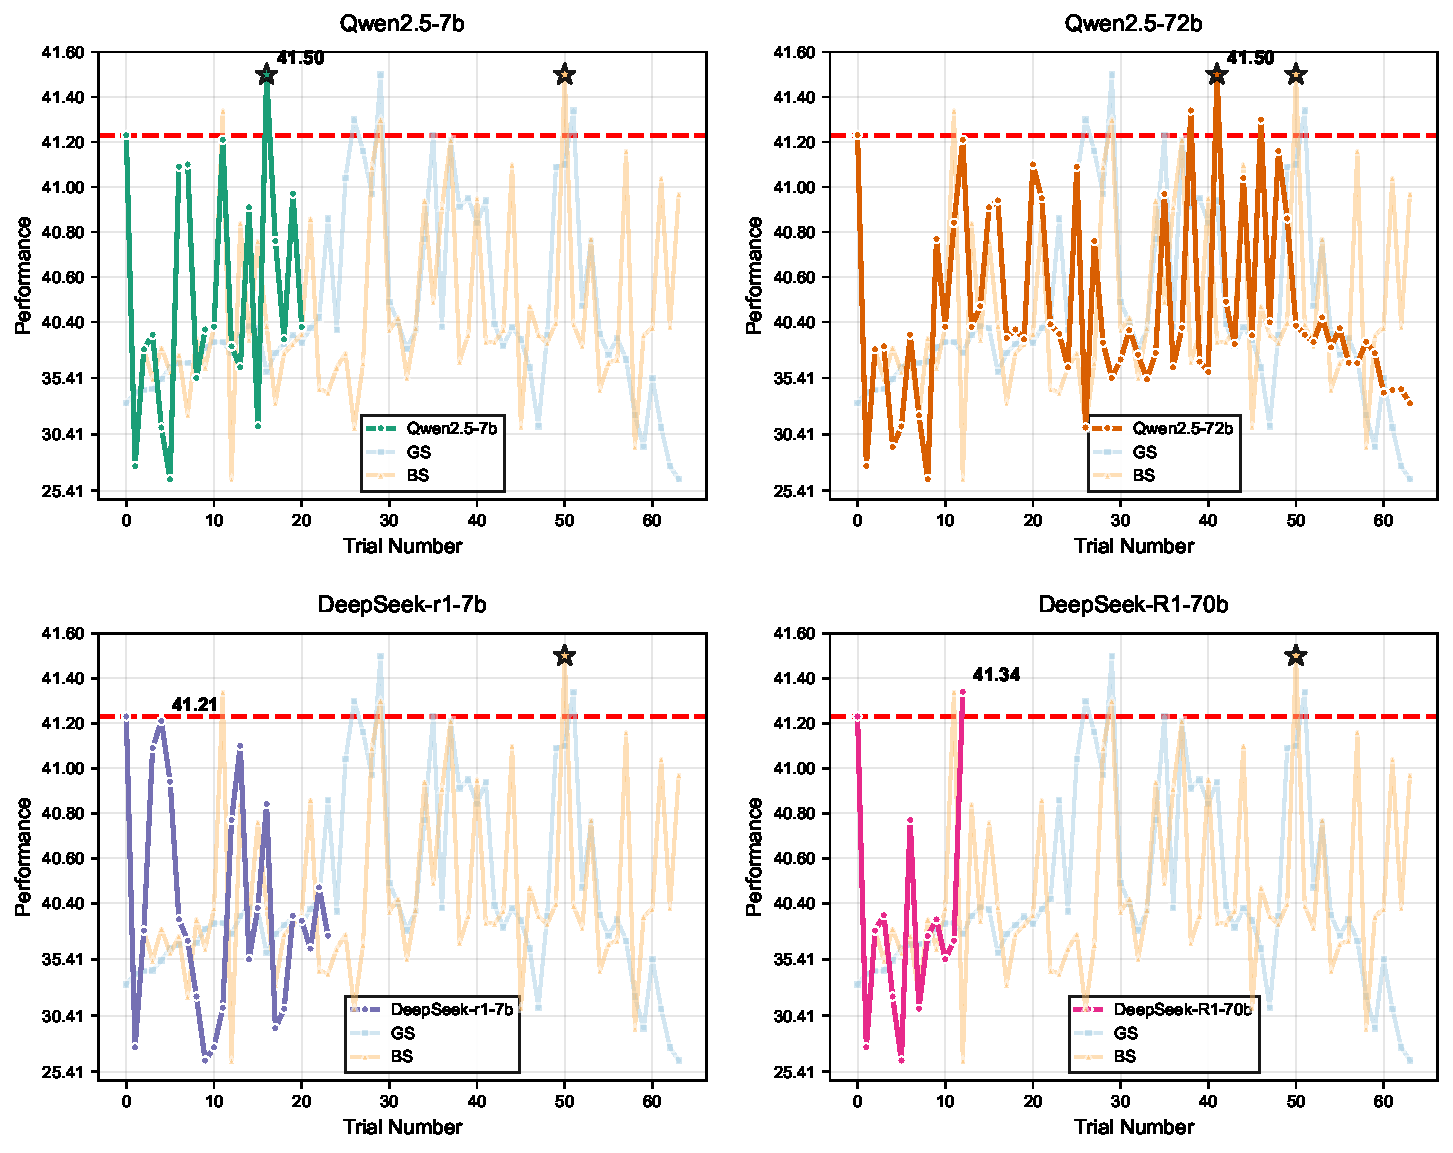
\includegraphics[width=1.0\linewidth]{figures/analysis/solver_comparison_Image_Completion.pdf}
    \caption{Failure Cases for the DeepSeek-R1 Family in the scientific computing field. Both DeepSeek-R1-7B and DeepSeek-R1-70B fail to reach the optimal results, marked with a star symbol ($\star$). Notably, DeepSeek-R1-7B fails to improve beyond the initial results, as indicated by the red dotted line, suggesting limited exploration capability in the search space.
    }
    \label{fig:failure_case}
\end{figure}